% AEJ-Article.tex for AEA last revised 22 June 2011
\documentclass[PP]{AEA}

%%%%%% NOTE FROM OVERLEAF: The mathtime package is no longer publicly available nor distributed. We recommend using a different font package e.g. mathptmx if you'd like to use a Times font.
\usepackage{mathptmx}

% The mathtime package uses a Times font instead of Computer Modern.
% Uncomment the line below if you wish to use the mathtime package:
%\usepackage[cmbold]{mathtime}https://www.overleaf.com/project/5de54d6638f785000167866a
% Note that miktex, by default, configures the mathtime package to use commercial fonts
% which you may not have. If you would like to use mathtime but you are seeing error
% messages about missing fonts (mtex.pfb, mtsy.pfb, or rmtmi.pfb) then please see
% the technical support document at http://www.aeaweb.org/templates/technical_support.pdf
% for instructions on fixing this problem.

% Note: you may use either harvard or natbib (but not both) to provide a wider
% variety of citation commands than latex supports natively. See below.

% Uncomment the next line to use the natbib package with bibtex 
\usepackage{url}
\urlstyle{same} % makes the font the same
\usepackage{natbib}
\usepackage{hyperref}
\usepackage{acronym}
\usepackage[names]{xcolor}
\usepackage{graphicx}
\usepackage{csvsimple}
% Uncomment the next line to use the harvard package with bibtex
%\usepackage[abbr]{harvard}
\usepackage{etoolbox}
\usepackage{geometry}
\usepackage{caption} % to re-use counters
\usepackage{threeparttable}

\newtoggle{fancy}
\togglefalse{fancy}

\newtoggle{draft}
\toggletrue{draft}
%\togglefalse{draft}

\newtoggle{final}
%\togglefalse{final}
\toggletrue{final}
%\iftoggle{final}{\togglefalse{draft}}{}


\iftoggle{draft}{
\usepackage{draftwatermark}
\SetWatermarkText{DRAFT}
\SetWatermarkScale{0.5}
\SetWatermarkLightness{0.85}%
}{\usepackage[final]{draftwatermark}}

\usepackage{xspace}
% to adjust floats
\usepackage{placeins}
% to read the table
\usepackage{booktabs}
\usepackage{ifthen}
\usepackage{csvsimple}
\usepackage{longtable}

\usepackage{textcomp}

\iftoggle{fancy}{
\input{fancy-config.tex}
}{}

\iftoggle{final}{
\usepackage[disable]{todonotes}
\newcommand{\misscitep}[2]{\citep{#2}}
\newcommand{\misscitet}[2]{\citet{#2}}
}{
\usepackage{todonotes}
\geometry{verbose,letterpaper,
	tmargin=1in,bmargin=1in,lmargin=1in,rmargin=2in}
\setlength{\marginparwidth}{1.9in}
\newcommand{\misscitep}[2]{\todo[color=green]{Missing citation: #1}{(\textcolor{red}{#2})}}
\newcommand{\misscitet}[2]{\todo[color=green]{Missing citation: #1}{\textcolor{red}{#2}}}
}



% This command determines the leading (vertical space between lines) in draft mode
% with 1.5 corresponding to "double" spacing.
\draftSpacing{1.5}

%% make somewhat tigher enumeration environments
\usepackage{enumitem}
\setlist[enumerate]{itemsep=0pt,parsep=0pt,topsep=1pt}
\setlist[itemize]{itemsep=0pt,parsep=0pt}

%% Acronyms
\acrodef{AEA}{American Economic Association}
\acrodef{DOI}{Digital Object Identifier}
\acrodef{FAIR}{Findable, Accessible, Interoperable, Re-usable}
\acrodef{PSID}{Panel Study of Income Dynamics}
\acrodef{HRS}{Health and Retirement Study}
\acrodef{RCT}{randomized control trial}
\acrodef{ICPSR}{Inter-university Consortium for Political and Social Research}
\acrodef{DCAP}{data and code availability policy}
\acrodef{PAP}{pre-analysis plans}
\acrodef{NACJD}{National Archive of Criminal Justice Data}
\acrodef{IAB}{Research Data Center (FDZ) at the Institute for Employment Research}
\acrodef{FSRDC}{Federal Statistical Research Data Centers}
\acrodef{FAQ}{frequently asked questions}
\acrodef{ReStud}{Review of Economic Studies}
\acrodef{EJ}{Economic Journal}
\acrodef{JASA}{Journal of the American Statistical Association}
\acrodef{CJE}{Canadian Journal of Economics}
\acrodef{AJPS}{American Journal of Political Science}
\acrodef{PII}{personally identifiable information}
\newcommand{\aeadcr}{AEA Data and Code Repository}

% reset colors
\definecolor{darkblue}{rgb}{0 0 255}
\hypersetup{colorlinks,
breaklinks,
citecolor=darkblue,
linkcolor=darkblue,
urlcolor=darkblue}

% Different ways to cite URLS
%\newcommand{\urlcite}[2]{\href{#1}{#2}
\newcommand{\urlcite}[2]{#2\footnote{\url{#1}}}
\newcommand{\purlcite}[2]{#2.\footnote{\url{#1}}}
\newcommand{\furlcite}[2]{#2 (\url{#1})}

%
% Periods covered by the report 
% Should be read in from R
\newcommand{\version}{Sun Dec 13 21:14:12 2020}
\newcommand{\firstday}{2019-12-01}
\newcommand{\lastday}{2020-11-30}
\newcommand{\jiraissues}{832}
\newcommand{\jiramcs}{509}
\newcommand{\jiraissuescplt}{715}
\newcommand{\jiramcscplt}{402}
\newcommand{\jiraexternal}{36}
\newcommand{\jiramcsexternal}{27}
\newcommand{\jiramcspending}{307}
\newcommand{\pkgsizemean}{1.72}
\newcommand{\mcpubtotal}{345}
\newcommand{\mcpubincmplt}{5}
\newcommand{\pppubnoncompl}{1}
\newcommand{\mcpubnoncompl}{1}
\newcommand{\pkgsizeq50x}{0.02}
\newcommand{\pkgsizeq90x}{6.47}


%\renewcommand{\firstday}{Dec 1, 2019}
%\renewcommand{\lastday}{Nov 30, 2020}

\begin{document}

\title{Report for 2020 by the AEA Data Editor }
\shortTitle{Report by Data Editor}
\author{Lars Vilhuber\thanks{%
Cornell University, lars.vilhuber@cornell.edu. }
}
\date{\today}
\pubMonth{May}
\pubYear{2020}
\pubVolume{--}
\pubIssue{--}
\JEL{}
\Keywords{reproducibility; replicability; science of science}




\maketitle

The \ac{AEA} Data Editor's  mission is to ``design  and  oversee  the  AEA  journals’  strategy for archiving and curating research data and promoting  reproducible  research'' \citep{10.1257/pandp.108.745}. The 2018 Report by the Data Editor \citep{10.1257/pandp.109.718} articulates how to implement that mission. Since July 2019, we have conducted comprehensive pre-publication reproducibility checks for all regular AEA journals, developed guidance for authors, and worked with peers at societies and groups in economics and elsewhere. 

Based on the experience from the first full year of reproducibility verification, we implemented several improvements in mid-2020. We provided improved guidance to authors depositing materials, clarified the \ac{DCAP}, expanded and clarified additional policies on third-party reproducibility checks, on post-publication updates to replication packages, and on required replication materials for field and lab experiments  (Section~\ref{sec:dcap}). We have reached out to numerous data creators and providers --- both authors who have created unique data resources, and commercial data providers that often provide the data for economic research --- and have discussed with these data providers access to data for reproducibility checks, mechanisms to request publication approval, and generally informed them of the need for reproducibility, provenance tracing, and transparency in economic research (Section~\ref{sec:producers}). 
We continue to coordinate with other journals, societies, and registries on these topics (Section~\ref{sec:coordination}).


\section{Updating the AEA Data and Code Availability Policy}
\label{sec:dcap}

After having introduced stronger principles of provenance and transparency into the  \ac{AEA}'s data and code availability policy in 2019 \citep{10.1257/pandp.110.dcap}, we monitored compliance and understanding as evidenced by the replication package submissions we received. It became quickly clear that stronger guidance, and greater clarity were needed to assist authors in complying with the \ac{DCAP}. Authors struggled with how best to document their code and data,  with the process of deposing data and code, and the ability to provide clear data provenance, including  data citations. We clarified the policy, and released the revised version in September 2020. The main content remains unchanged, but we simplified the main policy,  separated out the policy as applied to papers conducting (field and lab) experiments, and expanded the policy to encompass more clearly any primary data collection. We also introduced  supplementary policies that lay out how and when we expect reproducibility checks by third-parties to be conducted (also see \hyperref[sec:3rdparty]{our interactions with third-party verifiers}, and, as a logical consequence of more transparent data and code deposits, how to revise data and code deposits when post-publication changes become necessary. These policies are reprinted in \citet{10.1257/pandp.111.dcap} and accessible online at \url{https://www.aeaweb.org/journals/data}.

We also clarified the data and code availability policy as it applies to papers submitted to these Proceedings. All empirical and computational articles in the proceedings need to make code and data available in the same AEA Data and Code Repository as articles in the journals. However, other than verifying compliance with the policy (materials were deposited) and conducting basic checks (material can be read, metadata is in order), we do not conduct the same pre-publication reproducibility checks as we do for regular articles (see Section \ref{sec:compliance} for statistics on compliance).

But policies only outline what should occur, not how authors can achieve compliance. In order to assist authors in complying with the policy, thus improving turnaround times, we developed more detailed step-by-step guidance at \href{https://aeadataeditor.github.io/aea-de-guidance/step-by-step.html}{aeadataeditor.github.io/aea-de-guidance/step-by-step.html}. We also revised the information that authors need to provide when their manuscript is conditionally accepted (or, in some cases, during the review process). We have eliminated the duplicative requirement to provide  README files during the manuscript submission process --- they remain a required element in the data and code deposit process --- replacing it with a simpler form that requires authors to attest to compliance of their manuscript with the data citation requirement, provide details on where the data and code were deposited, and has them alert the Data Editor to any constraints on data access\footnote{The form is available at \href{https://www.aeaweb.org/journals/forms/data-code-availability}{aeaweb.org/journals/forms/data-code-availability}.} At the same time, the form provides hyperlinks to the guidance mentioned above. A simplified version of the form (reduced to a few checkboxes) is incorporated into the initial manuscript submission workflow. The primary goal of these forms and checkboxes is to alert authors to the need to comply with the policy early on, and hopefully leading to better compliance by the time that manuscripts are conditionally accepted. 

Furthermore, in collaboration with data editors at other journals in economics, management, and statistics, we have released a template README \citep{READMEv1.0.0} which helps authors compile all the information required for complete documentation of their data and code deposit.\footnote{The README is available at \href{https://social-science-data-editors.github.io/template_README/}{social-science-data-editors.github.io/template\_README/}.} With the publication of this report in the Proceedings, we will start verifying that authors use the README to document their replication package.


\subsection{Improving Findability of Replication Materials at the AEA}
\label{sec:findability}

Since the AEA began using a data and code repository hosted by \ac{ICPSR}, all deposits have JEL codes, and authors can add funder information and key metadata describing the data that is available within the deposit. Many authors avail themselves of this option. These attributes aid in making each deposit  findable through scholarly search engines such as \urlcite{https://clarivate.com/webofsciencegroup/solutions/web-of-science/}{Web of Science} and \urlcite{https://scholar.google.com/}{Google Scholar}. 

Deposits made prior to July 2019 and since migrated to the AEA Data and Code Repository do not have the rich metadata, since it must be entered interactively by authors. To improve the metadata of older deposits, we ran a campaign in summer and fall of 2020, thanks to the support provided by a research team at the University of Michigan and ICPSR. This campaign targeted several hundred papers, providing authors with a tool to augment the metadata associated with their deposits. A report on the success of the campaign is forthcoming, and the metadata provided by the authors is being incorporated as this report was being compiled. A second campaign will complete the work in Spring or Summer of 2021. 

Deposits receive their own \ac{DOI}, and can be cited in line with the Data Citation Principles \citep{Altman2013-fl,jddcp}. Authors are required to explicitly cite their data supplement if it contains original data; an entry in the references is automatically added in all cases. Conversely, the article that a supplement is associated with is clearly identified on the supplement's landing page. Future enhancements to the platform will be able to display other articles that also cite a supplement. 

We continue to verify that authors cite the datasets they have used and accessed, as required by the \ac{DCAP}, the AEA's citation requirements, and in line with the Data Citation Principles.  Data citations increase findability of data, allow data providers to receive proper credit, and align the Association with broader principles in the academic publishing world. The AEA's  \urlcite{https://www.aeaweb.org/journals/policies/sample-references}{Sample References} provide a style reference, and additional guidance for non-standard data sources, such as confidential or proprietary data, has been developed in collaboration with other journals and guidance by librarians.\footnote{\url{social-science-data-editors.github.io/guidance/addtl-data-citation-guidance.html}}.


\subsection{Third-party repositories}

The \ac{DCAP} allows for code and data deposit to be deposited at other trusted repositories, as long as all other elements of the \ac{DCAP} are complied with. In fact, authors are discouraged from duplicating deposits they have made elsewhere in the \aeadcr{}. This is intended to allow others to create replication packages prior to submitting at the AEA's journals, as a component of a reproducible workflow and possibly in compliance with funder data management policies. We have not observed many authors availing themselves of this possibility, with probably less than 10 deposits made in such a way. Authors wishing to deposit replication packages early in the research lifecycle are encouraged to consult the Social Science Data Editors website, where links to trusted repositories are provided.
	
\subsection{Post-publication modifications}

At the time of publication, the article is linked with one (or more) archived supplements, constituting the version of record. What happens when, despite pre-publication scrutiny, an error in the code emerges? The \ac{DCAP} provides for a \href{https://www.aeaweb.org/journals/data/policy-revisions}{clear policy}, identifying which modifications constitute a minor edit to the version of record, and which modifications lead to a higher version number, without modification of the existing version of record. In particular, any change that potentially changes a computational result or adds (untested) code will lead to a new version of the deposit being created, without changing or removing the version of record, even if the modifications fixes an error. However, the presence of replication packages that are newer than the version of record is signalled to readers via a banner, and is recorded in the metadata.

We have had few such post-publication updates. A handful of authors have requested that their historical migrated packages be updated, typically with an improved README. In a few cases, we had published incomplete replication packages when access to the code was not feasible due to COVID-19 related office closures. When authors regained access only after publication of the manuscript, the replication package was updated in a transparent fashion, compliant with our policy. 

\subsection{Intellectual Property and Licenses} 
\label{sec:ip}

For new deposits at the \aeadcr{}, authors retain  copyright. The default license for all repositories based at openICPSR is the  Creative Commons Attribution (CC-BY) \citep{CreativeCommons2017}, but authors can choose their own license,  though such licenses will be vetted by the Data Editor for compliance with the \ac{DCAP}. 

We see few authors deviate from the standard license. When deviating, authors tend to choose a different, open source license \citep{OpenSourceInitiative2018} for software and code. In a very small number of cases, we have worked with authors to publish data under more restrictive licenses, due mostly to ethical concerns, while ensuring that replication remains possible.

% Dwayne Benjamin, Toronto/P&P
% AER/FL Police officers

\subsection{Compliance}
\label{sec:compliance}

\begin{table}[t]
    \centering
    \caption{Compliance}
    \label{tab:compliance}
    \begin{threeparttable}
    \begin{tabular}{lccc}
    \toprule
         & Compliant & Incomplete & Non-compliant \\
    \midrule
    Papers and Proceedings &  87    &  4 & 1\\
    AER and journals       & xx    &  1  & 0\\
    \bottomrule
    \end{tabular}
    \begin{tablenotes}
    \footnotesize
    \item[] \textit{Note}: Unit of observation are manuscripts assessed between \firstday{} and \lastday{}. ``Incomplete" means the data deposit has not been completed, though the article has been published. ``Non-compliant" means that code or other required materials have not been provided.
    \end{tablenotes}
    \end{threeparttable}
\end{table}


We note that authors can be compliant with the policy without providing a copy of data used, as long as the reason for the inability to provide the data is acceptable, correct, and documented as part of the replication materials. 

Compliance with the policy (Table~\ref{tab:compliance}) has been excellent. In some cases, we have requested data that was not initially provided, when such data could be legally and ethically provided; by the second round of assessments, compliance was generally achieved (see also our discussion of outreach to data providers). In a very small number of cases, authors having conducted research in restricted-access data environments did not provide code. In several cases, relying on personal experience or by reaching out to the managers of the restricted-access environment, we were able to inform the authors of their ability to provide code, in compliance with any security requirements of the restricted-access data environment. In several cases, authors were unable to access the restricted-access environment due to COVID-19 lockdowns, which we accommodated in various ways; however, in all cases, code was ultimately provided. For a very small number of articles, compliance was achieved after the manuscript had been published. We are aware of only one case where the authors were unable to provide code because their employer asserted copyright and did not give permission to post code. One case in which the manuscript has been published is currently pending corrections by the authors, and has not been published as of \today, one month after publication of the article.

\begin{center}
    No changes beyond here
\end{center}

\section{Infrastructure for Verification of Reproducibility}
\label{sec:infrastructure}

The Data Editor manages the infrastructure needed to access data and code, conduct reproducibility checks, and archive and preserve replication packages. The first two points are provided by the replication team at Cornell University, the latter primarily by the  \aeadcr{} provided by openICPSR at the University of Michigan, with additional support from the AEA's in-house IT staff. 


\subsection{Pre-publication verification of computational reproducibility}
\label{sec:verification}


\begin{quote}
Report on articles (manuscript ID), reports (unique issues = tasks) and published repositories (only when tied to an article, requires transforming manuscript ID into DOI and querying crossref). Redo analysis from 2019.

\end{quote}

\paragraph{The process}

Pre-publicaton verification is conducted by the Data Editor's team at Cornell University. 
Requests for assessment of reproducibility are received, assigned to a team member, who then assesses data availability and compliance with requirements. When some data is available, a full or limited reproducibility check is conducted. If we cannot obtain access to the data or computational resources in a timely fashion, we may reach out to third-parties who can, and request a reproducibility check from them. Once all computations have been completed, a process that can take anywhere from a few minutes to several weeks, a report is compiled, reviewed and approved by the Data Editor, and submitted back to journal editors, who handle most communications with the authors. The report will have  one of four possible recommendations (see Table). A ``conditional acceptance'' implies that a revision will need to be resubmitted to the Data Editor to address any identified shortcomings. An ``acceptance'' means that no further changes are necessary, and both the manuscript (after copy-editing) and the replication package can be scheduled for publications.%
%
\footnote{Manuscript and replication package are generally published at the same time, though at the request of either editors or authors, the replication package can be published at any time after acceptance.} 
%
However, to streamline processing, we may also recommend an ``acceptance with modifications requested.'' In such a case, the remaining modifications are minor, and can be handled during copy-editing (for instance, a small number of tables need minimal changes) and prior to publication of the replication package (for instance, a fixable error in a program, or a clarification in the README, not affecting any important tables or figures). We have increasingly made use of this feature. While we monitor that authors comply with the request for modifications, no further computational assessment is made. Finally, we may recommend a ``revise and resubmit'' when serious issues have been identified that materially affect the conclusions of the manuscript. In the past year, two manuscripts required conversations with the editors and the authors, and both were resolved to the satisfaction of all involved.

\begin{table}[t]
    \caption{Response options for recommendations}
    \label{tab:responses}
    \centering
    \begin{tabular}{lr}
    \toprule
               & Frequency \\
               \midrule
        Accept &  \\
        Accept with changes &\\
        Conditional accept &\\
        Revise-and-resubmit & \\
        \bottomrule
    \end{tabular}
\end{table}

\paragraph{Reproducibility reports}

Between \firstday{} and \lastday{}, the AEA Data Editor team  received
\jiraissues{} requests,  for \jiramcs{} manuscripts.%
%
\footnote{This includes only requests submitted between those dates, and does not take into account in-progress requests on \firstday{}.}
%
Requests typically are channeled to the team by the AEA's journal submission and review system, but others were initiated by authors or editors directly, often while preparing the replication materials. Of these,  \jiraissuescplt{} reports (\jiramcscplt{} manuscripts) were submitted back to editors,\footnote{The balance are either in progress or are not coded in the adminstrative system as having been submitted to ScholarOne, such as replication packages for Papers and Proceedings.} and \jiramcspending{} were completed up to the point of publication of the data deposit, including any post-acceptance modifications.  Table~\ref{tab:jirastats} breaks these numbers down by journal.
%

\begin{table}[]
    \caption{Stats}
    \label{tab:jirastats}
    \footnotesize
    \begin{threeparttable}
    \centering
    
% Table created by stargazer v.5.2 by Marek Hlavac, Harvard University. E-mail: hlavac at fas.harvard.edu
% Date and time: Thu, Feb 18, 2021 - 01:40:43 PM
\begin{tabular}{@{\extracolsep{5pt}} lccccccc} 
\toprule 
        & \multicolumn{3}{c}{Requests} & \multicolumn{4}{c}{Manuscripts}\\
\cmidrule{2-4}\cmidrule{5-8}

Journal & (rcvd) & (cplt) & (external) & (rcvd) & (cplt) & (ext.) & (pend.) \\ 
\midrule 
AEJ:Applied Economics & 111 & 107 & 3 & 63 & 60 & 3 & 42 \\ 
AEJ:Economic Policy & 122 & 115 & 13 & 70 & 65 & 8 & 51 \\ 
AEJ:Macro & 131 & 126 & 3 & 67 & 64 & 2 & 46 \\ 
AEJ:Micro & 81 & 78 & 4 & 45 & 44 & 3 & 33 \\ 
AER & 182 & 176 & 12 & 108 & 103 & 10 & 80 \\ 
AER:Insights & 56 & 55 & 0 & 31 & 31 & 0 & 26 \\ 
JEL & 33 & 31 & 1 & 18 & 17 & 1 & 16 \\ 
JEP & 28 & 27 & 0 & 19 & 18 & 0 & 13 \\ 
\bottomrule 
\end{tabular} 

    \begin{tablenotes}
    \item[] \textit{Notes:} Data for requests received between \firstday{} and \lastday{}. AEA P+P do not generate a report, and are thus not counted under completed (cplt). (pend.) indicates that a manuscript has been marked ready for publication, and may have been published (separate report forthcoming).
    \end{tablenotes}
 \end{threeparttable}
   \end{table}


\paragraph{Third-party replicators}

A total of \jiraexternal{} issues were sent to external parties with requests for verification (this includes revisions), for \jiramcsexternal{} manuscripts (see Table~\ref{tab:jirastats} for statistics by journal, Appendix~\ref{app:3rdparty} for a list of third-party replicators). We appreciate the willingness of all third-party replicators to provide us with their time and effort in reproducing papers. In particular, \href{https://cascad.tech}{cascad}, a French reproducibility certification agency, generously provided us with 21 reports.



\begin{table}
    \centering
%    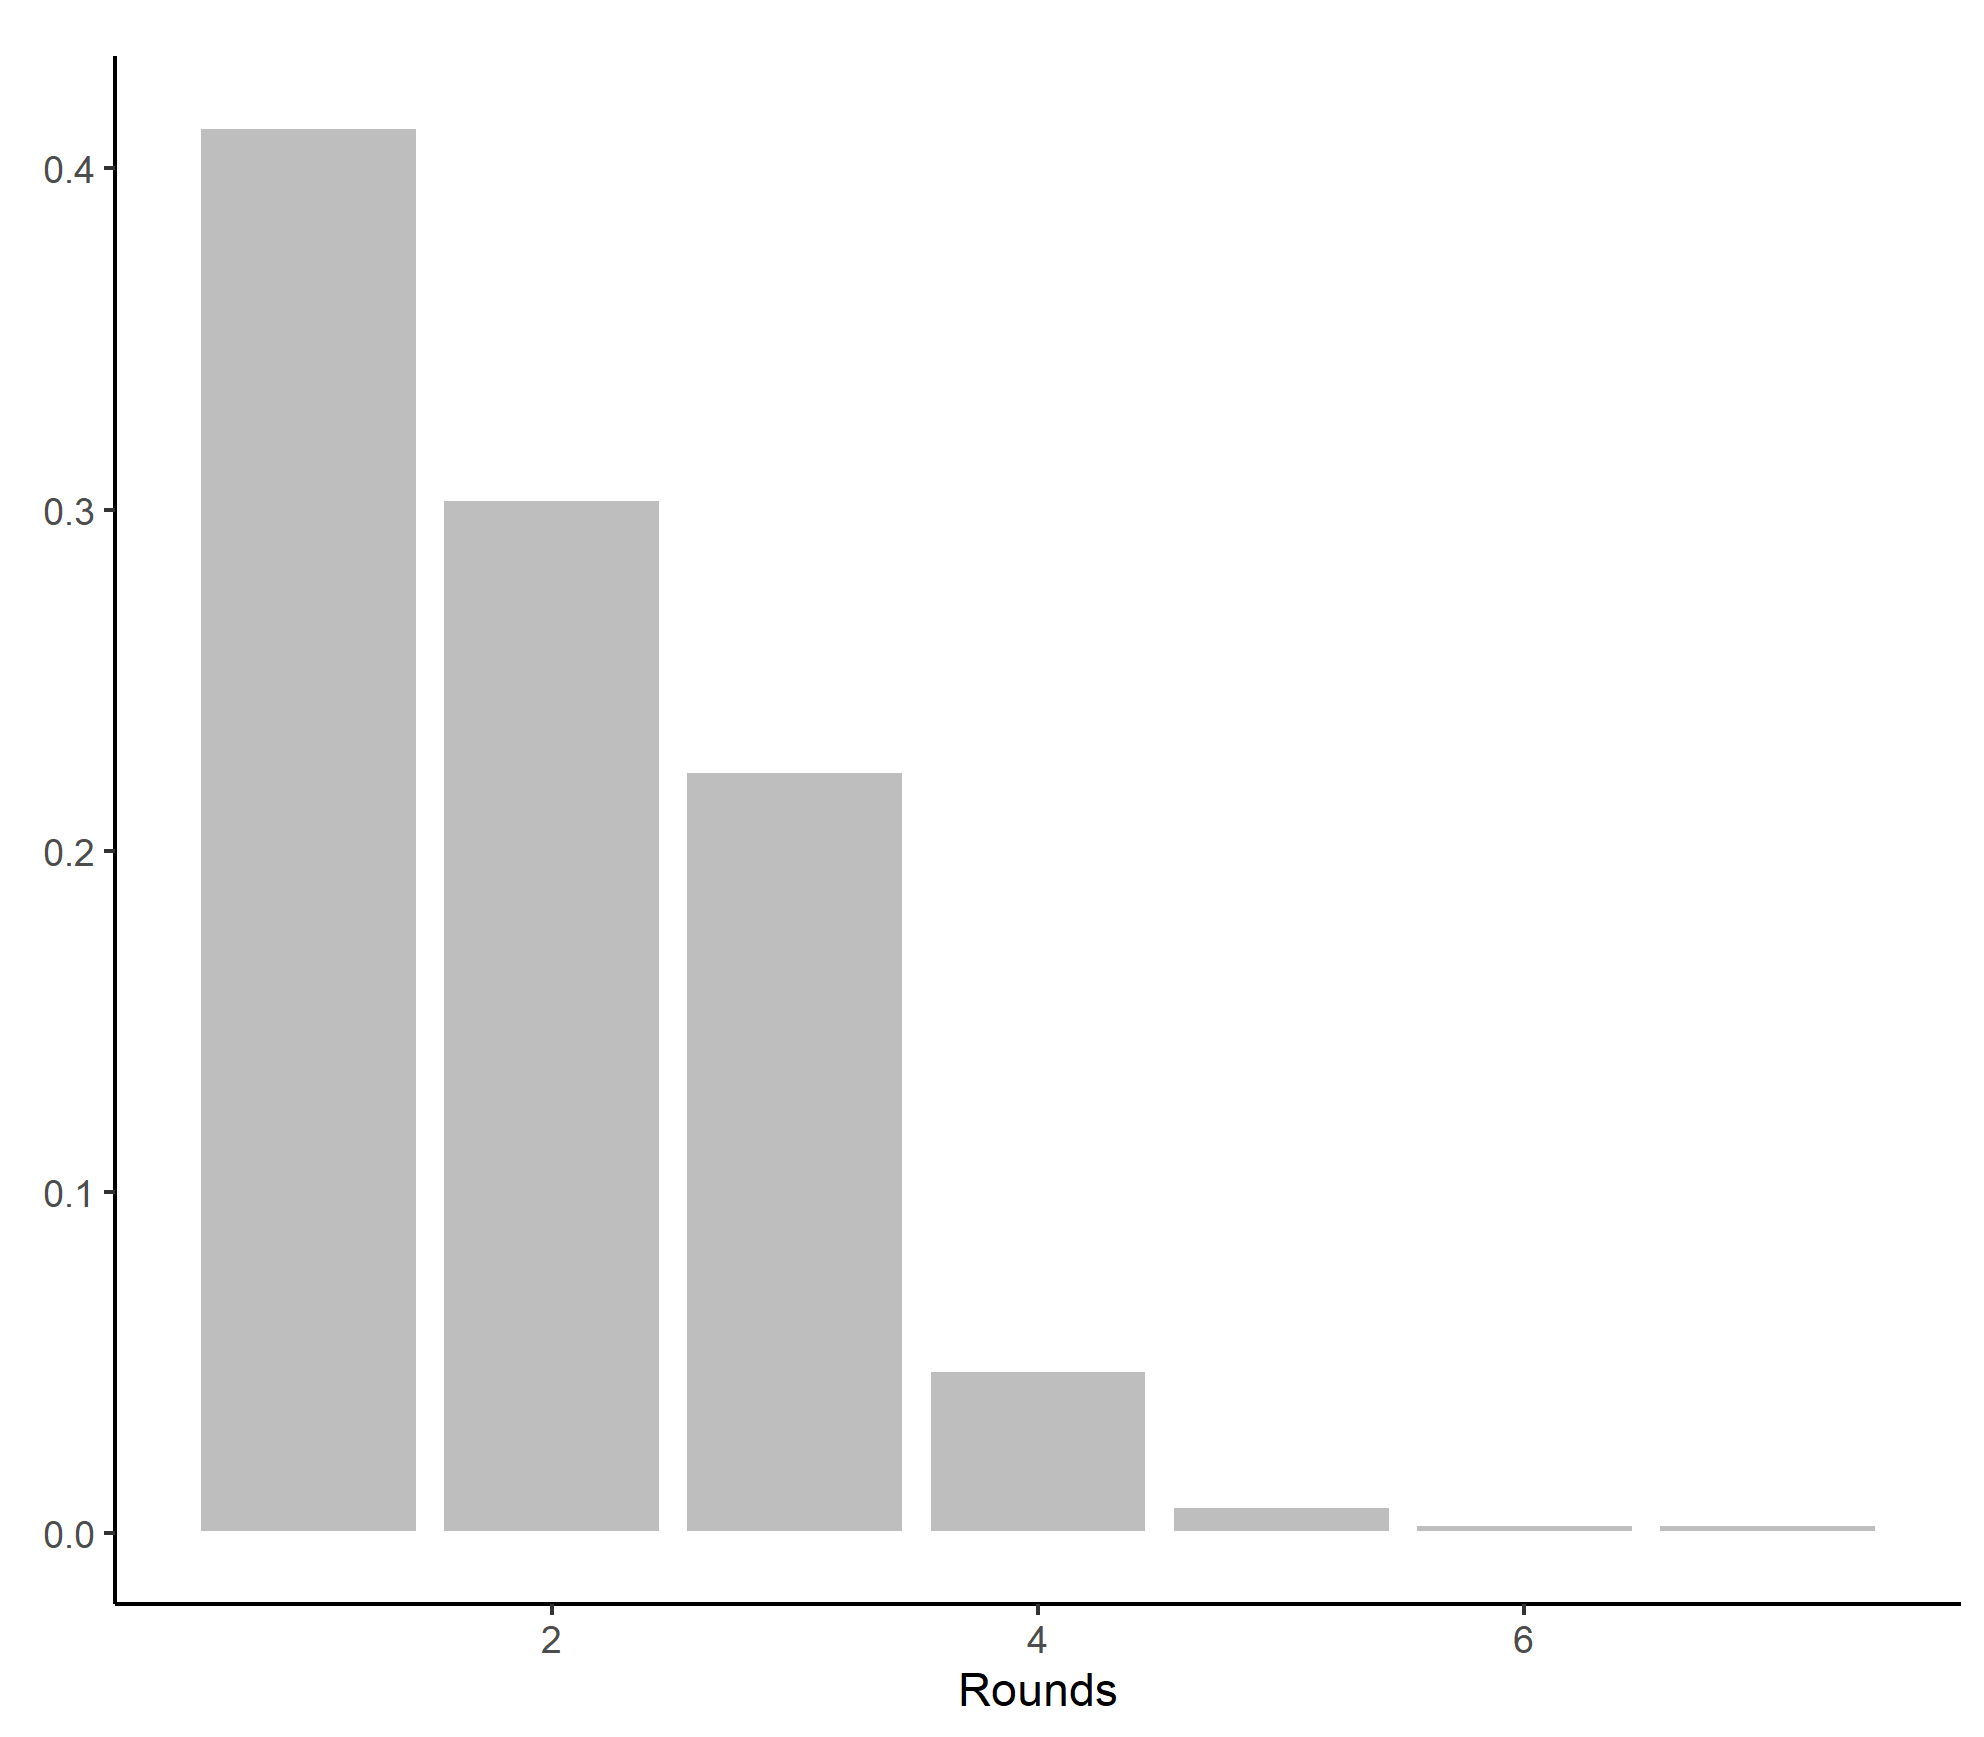
\includegraphics[height=0.4\textheight]{images/n_rounds_plot.png}
    See Liz Braunstein's tables - the final publication will have these numbers.
    \caption{Assessment rounds for completed manuscripts}
    \label{tab:pre:rounds}
\end{table}

\begin{table}
    \centering
%    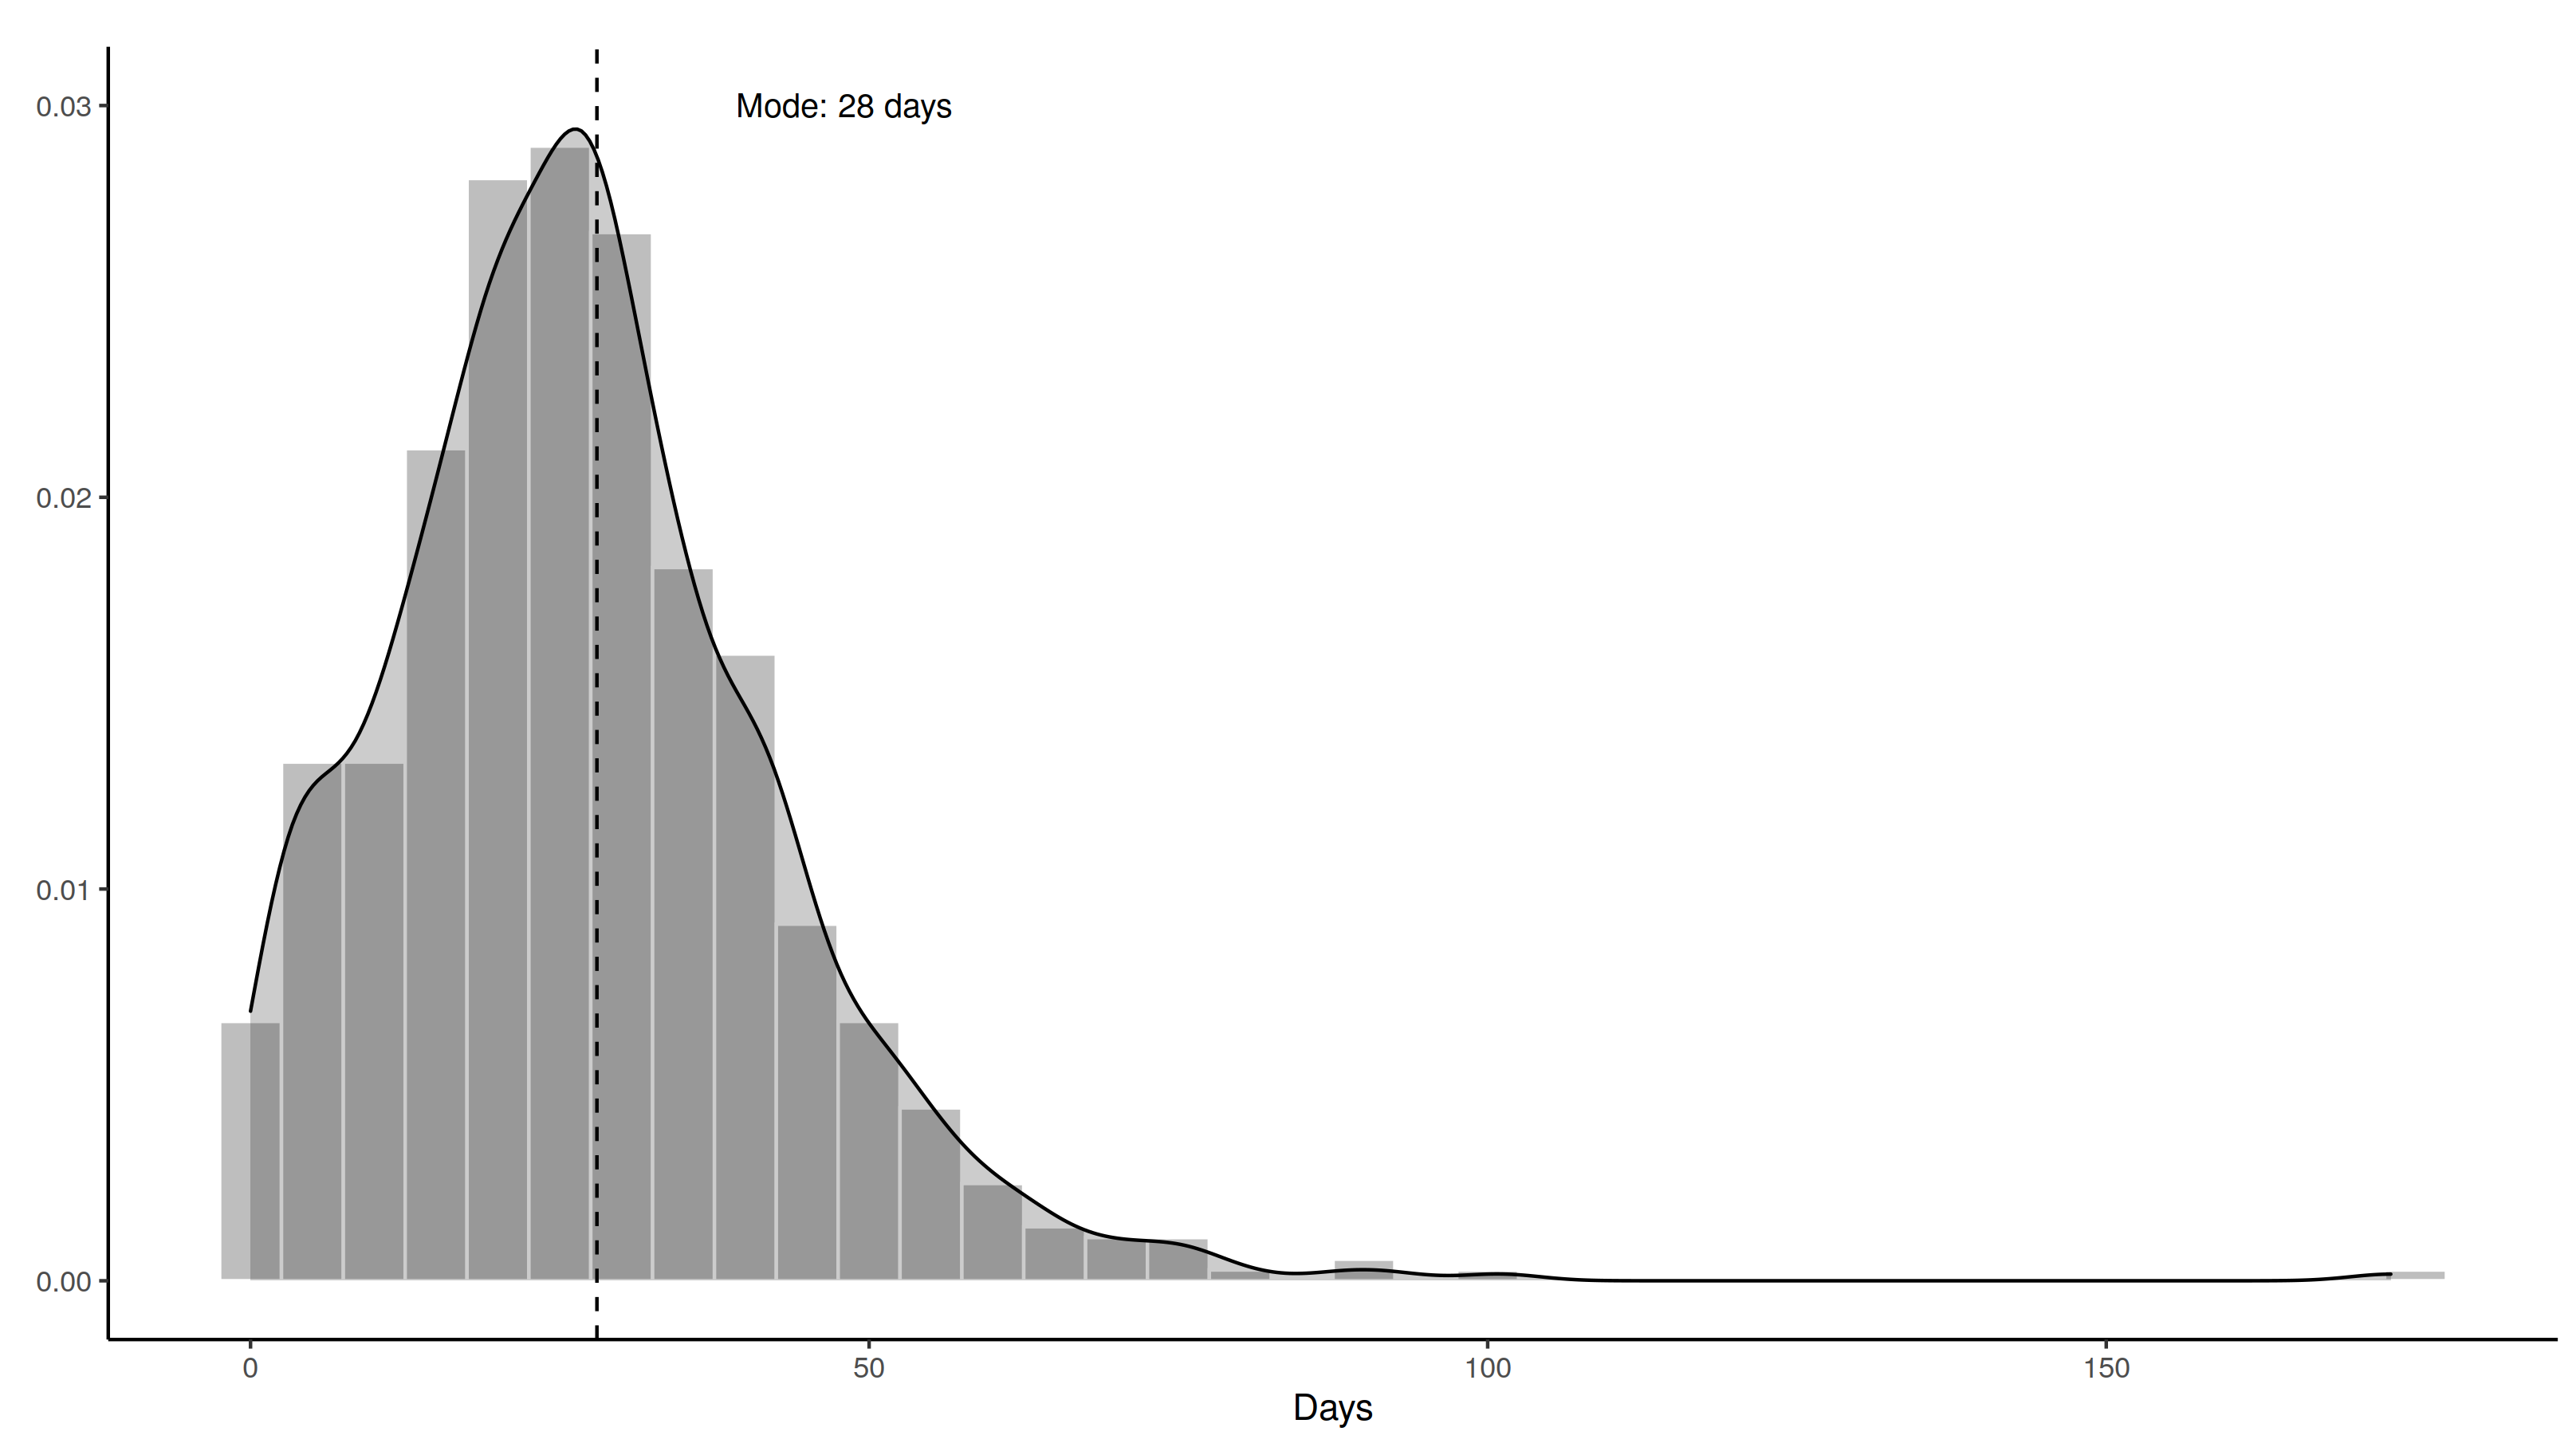
\includegraphics[height=0.4\textheight]{images/revision_round_length_hist.png}
See Liz Braunstein's tables - the final publication will have these numbers.
    \caption{Length of an assessment round in days}
    \label{tab:pre:round_length}
\end{table}


\paragraph{Frequent issues}

We provide a heuristic overview of notable issues  encountered when attempting to reproduce results. We note that none of the \jiramcs{} manuscripts we assessed had  fundamental flaws --- all problems identified so far have been fixable (and fixed). 

\subparagraph{Computational issues:}  We still encounter mostly preventable issues of computational instability (see \citet{mccullough_numerical_1999} for one of the earlier observations in this vein). In most cases, authors fail to set a random seed, though this is a requirement of the policy. In some cases, differences in software versions can generate numerical differences despite having fixed a pseudo-random seed generator, for instance optimization routines in Matlab\footnote{\href{https://it.mathworks.com/matlabcentral/answers/422349-fmincon-in-new-matlab-version-gives-different-results}{mathworks.com/matlabcentral/answers/422349-fmincon-in-new-matlab-version-gives-different-results}} and Julia v1.5's faster random number generator.\footnote{\href{https://web.archive.org/web/20201216032133/https://docs.julialang.org/en/v1/NEWS/}{docs.julialang.org/en/v1/NEWS/}} We have also run into issues when Fortran compilations require specific versions of libraries, when versions of \href{https://www.dynare.org/}{Dynare} are not backward-compatible, or when simple data import (Stata) or export (Matlab) functionality does not work the same way on different operating systems. In the past year, we did not encounter use of newer technologies such as ``containers,'' and almost never the use of ``manifest''-like files in R, Python, and Julia, which alleviate some of these issues.  

\subparagraph{Incomplete instructions and manual manipulation:} While mechanisms such as \texttt{make} files and similar systems have been in use in software development for decades, they are very rarely used in replication packages in economics, even when it would seem a natural fit (Fortran compilations). We have encountered very manual (and tedious) instructions on how to assemble a compilable project for Fortran code, or how to generate a map using GIS software, despite the availability of reproducible tools in all cases. We encountered instructions to repeatedly change small parameters in multiple places in code prior to recompilation, or to manually move datasets between two directories, when the use of parameter files, function calls, or relative directory paths are basic mechanisms of programming. These inefficient mechanisms, while at least initially tolerated, are not just wasteful of replicator time, they are an inefficient use of the author's time as well, and can (and has) lead to errors being introduced into the manuscript's tables and figures. 

\subparagraph{Incomplete data provenance and data availability:} Most articles still provide imprecise or incorrect information regarding access to data that is not provided. In some cases, authors fail to provide data that should be provided, in other cases, authors inadvertently provide data for which they do not have redistribution rights. 

\paragraph{Delays} 

A recurring concern expressed by editors and staff members are delays in publication, due to the verification process. Table~\ref{tab:pre:rounds} shows that the median number of times a manuscript is reviewed by the AEA Data Editor is 2 - far too few manuscripts are given a rating of "acceptable" upon first pass. This leads to substantial time before the manuscript can proceed to copy-editing. We are currently making an analysis of the total time to publication (not yet available).

\paragraph{Process improvements}

In order to increase the initial acceptance rate, we set out in Summer 2020 to review the entire process that authors face. We made several changes aimed at (a) providing authors with the information as early as possible, when it is still easy to include reproducible practices in projects at relatively low cost and (b) providing authors with better information, to reduce frictions and uncertainty. As noted  \hyperref[sec:dcap]{earlier}, we introduced informational forms upon submission, and a brief required information sheet with links to updated and detailed guidance on how to prepare and submit replication packages. We also provide links to the reproducibility checks that our team uses, so authors know in advance what checks will be applied to their replication package. These changes were rolled out in September 2020, but have not yet been incorporated into all journal communications. Finally, the new template README \citep{READMEv1.0.0} introduced in December 2020 with other data editors will hopefully also reduce uncertainty and increase the completeness of the information. 


\subsection{Migrating Historical Supplements}
\label{sec:migration}

We initially migrated the bulk of historical data (and code) supplements, from ZIP files stored on AEA servers to the \aeadcr{}. As noted earlier, for many of these deposits, we have successfully requested assistance from several hundred authors to update the metadata, improving presentation and findability. A few hundred replication packages are still pending migration, pending reconciliation of duplicates and large-file limitations. Upon demand from readers, we have also sometimes reached out to authors to request materials from articles which were published prior to the original publication of a data availability policy. 

% report on UMich metadata project
% data provided by email

Thanks to support from a research team at the University of Michigan, we were able to enlist the aid of authors of migrated replication package to improve the attached metadata.  As part of the project, we sent 8,538 email to 3,005 authors of 1,460 studies. Out of the 1,000 authors (35\%) who responded, 911 (30\%) provided additional metadata for 522 studies. An article is expected at the conclusion of the experiment.

\subsection{Improving the \aeadcr{}}
\label{sec:improvingaeadcr}

We continually assess the technical performance of the \aeadcr{}. In collaboration with ICPSR, we have increased the default quota from 2GB to 30GB, streamlining the ability of researchers to deposit large replication packages.\footnote{It was previously possible to deposit large replication packages greater than 2GB, but required manual adjustments, resulting in delays and occasionally confusion.} A new workflow has been developed, which provides greater clarity to journal managers on the back-end, and prevents errors that users frequently made. It lays the groundwork for further enhancements in the future. 

% distribution of sizes - email from Jared

\begin{figure}[t]
    \centering
    %\includegraphics{} 
    PLACEHOLDER - 
    \caption{Size distribution of replication packages deposited between  \firstday{} to \lastday{}}
    \label{fig:size_packages}
\end{figure}



\section{Working with Other Providers of Scientific Infrastructure to Improve Support for Documenting Provenance and Replicability}
\label{sec:coordination}

An important component of the AEA Data Editor's position is to interact with other providers of scientific infrastructure. This involves other publishers and journals, archives such as ICPSR, providers of restricted or proprietary data, the AEA RCT Registry, metadata harvesters, and third-party verification services. 

\subsection{Highlighting Data Resources}

While reviewing replication packages, we occasionally identify data, prepared in the course of the research, which could be of greater value if separately archived and professionally curated. This may be because of significant value-added, or because the data would have been difficult to access, if not for the author's data collection or data preparation efforts. Examples include digitized maps of India made amenable for GIS software \citep{10.1257/aer.20171673} or historical Economic Census data for the United States \citep{ganapati2020}. These data are then processed by professional data librarians at ICPSR, and ultimately made available to the broader research community via the regular (non-AEA) ICPSR repository, while providing proper attribution to the author. The collaboration of the authors is voluntary, and we appreciate their efforts. Authors who believe that their data is unique and of value should contact the AEA Data Editor early enough in the research process, even when acceptance at the AEA journals may be uncertain. 

\subsection{Data Providers}
\label{sec:producers}

We regularly meet and communicate with academic and commercial data providers, on behalf of specific authors or because we have identified a data provider as a frequently used resource. Discussion topics include making data citations easier, clarifying licenses, requesting blanket or streamlined data redistribution authorizations, or suggesting improved curation of data to avoid repeatedly copying data from uncurated websites to the curated \aeadcr{}. As an example, after an email exchange with the leadership of the Economic Policy Uncertainty website \citep{10.1093/qje/qjw024}, the website changed its license to a liberal Creative Commons license, which allows broad re-use and facilitates reproducibility.

In the course of the past year, we have talked about some or all of these topics with IPUMS, EPU, the UNCTAD Division on International Trade and Commodities (TRAINS data), the World Bank, Standard and Poor's, Bloomberg, Tick Data, Haver Analytics, Federal Reserve of St. Louis data librarians\footnote{I am indebted to  Adrienne Brennecke at the St. Louis Fed, who facilitated many of these conversations.}, the World Management Survey, Ben Zipperer at the Economic Policy Institute, Jim Poterba and Dan Feenberg at the NBER, Lucia Foster (U.S. Census Bureau), Barbara Downs (U.S. Census Bureau and Federal Statistical Research Data Centers), the Research Data Centre (FDZ) of the German Federal Employment Agency (BA) at the Institute for Employment Research (IAB), the German Research Data Center of the SOEP, Research Data Center of the German Pension Insurance, the UK Data Archive, the Ministério da economia do Brasil, and the French Centre d'accès sécurisé de données (CASD). 

\subsection{Economics Journals}

We continue to coordinate with other data editors conducting similar activities at other journals. An informal mailing list managed by the AEA Data Editor is used occasionally to interact with others.\footnote{Journal editors wishing to join the mailing list should contact the AEA Data Editor.} Mailing list members who wish to be more actively involved can participate in the development of the \urlcite{socialsciencedataeditors.github.io}{website of the S ocial Science Data Editors}. The website contains guidance on data citations and data availability statements, best practices for coding and data preparation, and links to various tools useful to replicators. The recently released template README is one example of collaboration, having benefited from contributions from Miklos Kóren (\ac{ReStud}), Joan Llull (\ac{EJ}), Peter Morrow and Marie Connolly (\ac{CJE}), Chris Paciorek (JASA), Ben Greiner (Management Science),  Kevin Lang (JOLE), Harald Uhlig (JPE). A somewhat newer group emerging from a group of data repositories at Data-PASS has also initiated a mailing list called the Journal Editors Discussion Interface (\urlcite{https://dpjedi.org/}{JEDI}).


\subsection{Third-party verification services}
\label{sec:3rdparty}


We continue to rely on and have discussions with third-party verification services. As noted earlier, \jiramcsexternal{} reports were provided by some sort of external replicator. Of those, several were provided by institutions that already are organized as a reproducibility service (R-squared at Cornell University, cascad in France). The AEA Data Editor has had preliminary discussions with several institutions about the interest and possibilities of formalizing such services. Issues of cost, frequency, and at what point such services would be involved in the research lifecycle remain unresolved. 



\section{Working with the Economics Community to Enhance and Broaden Education on Replicable Science}

We have already noted the outreach to other journals and repositories above. Educating the current and future generations of economists is one of the longer-term goals for improving reproducibility of research. The AEA Data Editor has presented at TIER, and at various regional economics conferences that connect to communities of junior and later-career economists. One of the successful CSWEP "Fireside chats" is scheduled with the AEA Data Editor in late January. Various recordings of such presentations by the AEA Data Editor are available on Youtube. Together with BITSS (UC Berkeley), a framework and platform to support teaching reproducibility is being developed, complementing other existing services such as the ReplicationWiki. Presentations at the CTREE conference are planned. 

\section{Data and Code Availability Statement}
\label{sec:dcas}

All data and code used to generate figures and tables in this article can be found at TBD.

\FloatBarrier
% Remove or comment out the next two lines if you are not using bibtex.
%
% NOTE: Do not modify the AEADataEditor.bib manually!
%
\bibliographystyle{aea-mod}
\bibliography{paper,references}

% The appendix command is issued once, prior to all appendices, if any.
\appendix

%\input{appendix.tex}

\section{Replication team at Cornell University}
\label{app:replicators}

The following students have provided excellent assistance in reproducing the results from the \jiramcs{} articles processed by the Replication Lab:
%
% Provided by Melissa on 2020-12-18
%
Ololade Omotoba,
Craig  Schulman,
Daniella Pena,
Jeong Hyun Lee,
Jiayin Song,
Jill Nicole Crosby,
Joshua Gil Passell,
Julia R Zimmerman,
Justin Sun,
Lauren  Stubbs,
Kate  Hofer,
Kirubeal  Wondimu,
Liam Cushen,
Louis Liu,
Luis  Lopez Cabrera,
Lydia Reiner,
Manas Kumar Gogula,
Mary-Jo  Ajiduah,
Matt H Wang,
Melanie Chen,
Nehedin  Juarez,
Franklin Omullo,
Peter Rafael Sanchez,
Rubal Mistry,
Naomi  Li,
Ryan Ali,
Seong Hwan Kim,
Siyang Yu,
Steve Yeh,
Syon Verma,
Tarangana Thapa,
Valerie  Setiawan,
Weilun Shi,
William  Silverman,
Xiangru Li,
Ximei Shen,
Yanyun Chen,
Yuan-Hsuan Lin,
Zebang Xu,
Zechariah  Karsana,
Zhaojiahong Zhu.


Graduate students David Wasser, Meredith Welch, and Hyuk Harry Son (all Cornell University) and Research Aide Michael Darisse (Cornell University) have been invaluable assistants in training and coordinating the work as well as developing the methods and procedures which we have made public. 

\section{Third-party replicators}
\label{app:3rdparty}

We are grateful to the following third-party replicators (individuals\footnote{We do not name individuals when doing so would reveal information not already known to the manuscript's authors, naming the institution instead.} and institutions, in no particular order) who assisted us with verifications when we were unable to access data or, in some cases, computing resources:
%
Peri Weisberg (San Francisco Human Services Agency), Research Data Centre (FDZ) of the German Federal Employment Agency (BA) at the Institute for Employment Research (IAB), Majken Stenberg, CHRR at The Ohio State University, Florio Arguillas at the Results Reproduction (R-Squared) service at Cornell University, Kan Yao (Yale University),  Yulia Zhestkova (University of Chicago), Kamen Velichkov (Wharton), Ian Schmutte (University of Georgia), Paulo Guimarães (Banco de Portugal Microdata Research Laboratory - BPLIM), Arpita Patnaik (University of Wisconsin), Joint Committee on Taxation of the Congress of the United States, Upjohn Institute (2x), Kevin McKinney (U.S. Census Bureau), Vítor Costa (Cornell University, 2x), Rahul Kasar and Andrea Garcia (Federal Reserve Board). We in particular want to thank Olivier Akmansoy, Christophe Hurlin (Université d'Orléans), and Christophe Pérignon (HEC Paris), all of \href{https://cascad.tech}{cascad}, a certification agency for scientific code and data, who have been generous of their time and resources, and have provided us with 21 reports. They have been able to leverage their access to confidential French administrative data (customs and labor market data), and have served as our proxies when data access was only available to European residents for Swedish administrative data. 

We thank the following individuals who provided us with direct access to data and computing resources under their control, in order to prepare a reproducibility report. In such cases, we were able to conduct our checks ourselves, with full independence: Marc-Andreas Muendler (UCSD), Dan Feenberg (NBER).

We do not name the authors with whom we signed non-disclosure agreements, or who otherwise provided us with access to data that could not be published. We are grateful for their flexibility and patience.


\end{document}

